\documentclass[tikz]{standalone}
\newcommand{\printSQ}[3]{\filldraw [fill=#3, draw=black] (#1-0.5,#2-0.5) rectangle (#1+0.5,#2+0.5);}
\begin{document}
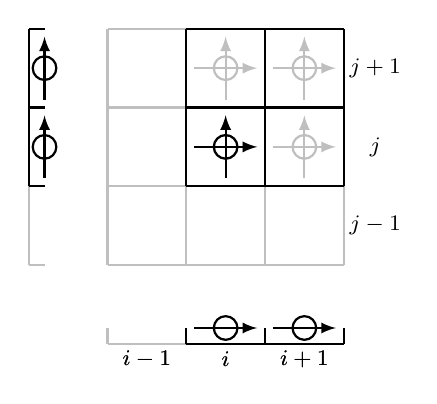
\begin{tikzpicture}[thick,scale=1,line join=round,>=latex]
  \footnotesize
  \foreach \i in {0,1,2,3} {
      \draw [color=lightgray] (0,\i) -- (3,\i);
      \draw [color=lightgray] (\i,0) -- (\i,3);
    }
  \foreach \i in {1,2,3} {
      \draw [color=black] (1,\i) -- (3,\i);
      \draw [color=black] (\i,1) -- (\i,3);
    }
  % \draw [color=blue!63, line width=3] (1.5,2) -- (2.052,2);
  % \draw [color=blue!63, line width=3] (2,1.5) -- (2,2.052);
  \foreach \i in {1,2} {
      \foreach \j in {1,2} {
          \draw [color=lightgray] (\i+0.5,\j+0.5) circle (0.15);
          \draw [color=lightgray,->] (\i+0.1,\j+0.5)--(\i+0.9,\j+0.5);
          \draw [color=lightgray,->] (\i+0.5,\j+0.1)--(\i+0.5,\j+0.9);
        }
    }
    \draw [color=black] (1+0.5,1+0.5) circle (0.15);
    \draw [color=black,->] (1+0.1,1+0.5)--(1+0.9,1+0.5);
    \draw [color=black,->] (1+0.5,1+0.1)--(1+0.5,1+0.9);
  
  % \draw (0.5,-0.2) node{$i-1$};
  % \draw (1.5,-0.2) node{$i$};
  % \draw (2.5,-0.2) node{$i+1$};
  \draw (3.4,0.5) node{$j-1$};
  \draw (3.4,1.5) node{$j$};
  \draw (3.4,2.5) node{$j+1$};
  
  \draw [color=lightgray] (0,-1) -- (1,-1);
  \draw [color=lightgray] (0,-1) -- (0,-0.8);
  \draw [color=black] (1,-1) -- (3,-1);
  \draw [color=black] (1,-1) -- (1,-0.8);
  \draw [color=black] (2,-1) -- (2,-0.8);
  \draw [color=black] (3,-1) -- (3,-0.8);
  \draw (1.5,-0.8) circle (0.15);
  \draw (2.5,-0.8) circle (0.15);
  \draw [->] (1.1,-0.8)--(1.9,-0.8);
  \draw [->] (2.1,-0.8)--(2.9,-0.8);

  \draw (0.5,-1.2) node{$i-1$};
  \draw (1.5,-1.2) node{$i$};
  \draw (2.5,-1.2) node{$i+1$};
  
  \draw [color=lightgray] (-1,0) -- (-1,1);
  \draw [color=lightgray] (-1,0) -- (-0.8,0);
  \draw [color=black] (-1,1) -- (-1  ,3);
  \draw [color=black] (-1,1) -- (-0.8,1);
  \draw [color=black] (-1,2) -- (-0.8,2);
  \draw [color=black] (-1,3) -- (-0.8,3);
  \draw (-0.8,1.5) circle (0.15);
  \draw (-0.8,2.5) circle (0.15);
  \draw [->] (-0.8,1.1)--(-0.8,1.9);
  \draw [->] (-0.8,2.1)--(-0.8,2.9);

  \draw (0.5,-1.2) node{$i-1$};
  \draw (1.5,-1.2) node{$i$};
  \draw (2.5,-1.2) node{$i+1$};
\end{tikzpicture}
\end{document}